\setproblem{25636}

\begin{frame}[label=p3]{소방차(25636)}

\tiny

\begin{block}{문제}
ANA 도시는 $N$개의 교차로와 $M$개의 양방향 도로로 이루어져 있고, 교차로는 $1$번부터 $N$번까지 번호가 매겨져 있다. $S$번 교차로에는 ANA 도시의 유일한 소방서가 위치하며, 무겸이는 이곳에서 소방차 운전 기사로 일하고 있다. 무겸이는 소방차를 타고 화재가 발생한 교차로에 출동해서 화재를 진압한다.

소방차에는 물을 담을 수 있는 물탱크가 있고, 이동 중에 교차로에 도착할 때마다 교차로에 설치된 소화전을 이용해 물탱크에 물을 충전한다. 소방차가 $i$번째 교차로에 한 번 도착할 때마다 충전하는 물의 양은 $a_i$리터이다. 소방차는 소방서가 위치한 교차로에서 출동할 때와 화재가 발생한 교차로에 도착했을 때에도 물을 충전한다. 물을 충전하는 데에는 시간이 걸리지 않으며, 물탱크의 용량에도 제한이 없다.

어느 날 $T$번 교차로에 화재가 발생했다. 무겸이는 소방차를 타고 $S$번 교차로에서 $T$번 교차로까지 \textbf{최단 경로}로 이동한다. 단, 최단 경로는 여러 개일 수 있다. 이때 무겸이는 여러 최단 경로 중에서 \textbf{물탱크에 담긴 물의 양이 최대가 되는 경로}를 선택한다.

무겸이가 $T$번 교차로에 도착했을 때 소방차의 이동 거리와 물탱크에 충전된 물의 양을 구하시오.
\end{block}

\begin{block}{입력}
첫째 줄에 교차로의 수 $N\ (2 \le N \le 100\,000)$이 주어진다. \\ 
둘째 줄에 $a_1, a_2, \dots, a_N$이 주어진다. $(1 \le a_i \le 1\,000\,000)$\\ 
셋째 줄에 도로의 수 $M\ (1 \le M \le 300\,000)$이 주어진다.\\ 
다음 $M$개의 줄에 도로 정보 $u, v, w$가 주어진다. $(1 \le u,v \le N,\ u \ne v,\ 1 \le w \le 1\,000\,000)$\\ 
마지막 줄에 소방서 위치 $S$와 화재 발생 교차로 $T$가 주어진다. $(1 \le S,T \le N,\ S \ne T)$\\
\end{block}

\begin{block}{출력}
$S$번 교차로에서 $T$번 교차로까지의 \textbf{최단 거리}와, 그 최단 경로들 중에서 \textbf{가장 많은 물을 모을 수 있는 경로의 물의 양}을 출력한다.  
만약 $T$번 교차로에 도달할 수 없다면 $-1$만 출력한다.
\end{block}

\end{frame}

\begin{frame}{예시 그래프}

\begin{center}
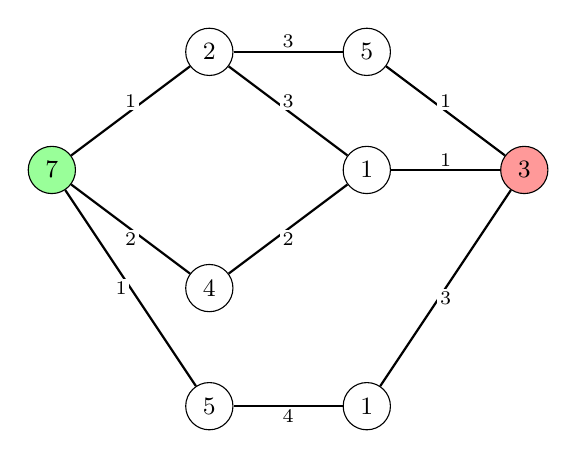
\begin{tikzpicture}[
    vertex/.style={circle, draw, minimum size=6mm, inner sep=0pt, font=\small},
    start/.style={circle, draw, fill=green!40, minimum size=6mm, inner sep=0pt, font=\small},
    goal/.style={circle, draw, fill=red!40, minimum size=6mm, inner sep=0pt, font=\small},
    edge/.style={thick},
    w/.style={font=\scriptsize, fill=white, inner sep=1pt}
]

% ---- nodes (value only) ----
\node[start] (1) at (0,0) {7};
\node[vertex] (2) at (2,1.5) {2};
\node[vertex] (3) at (2,-1.5) {4};
\node[vertex] (4) at (2,-3) {5};

\node[vertex] (5) at (4,1.5) {5};
\node[vertex] (6) at (4,0) {1};
\node[vertex] (7) at (4,-3) {1};

\node[goal] (8) at (6,0) {3};

% ---- edges ----
\draw[edge] (1) -- node[w,above] {1} (2);
\draw[edge] (1) -- node[w,below] {2} (3);
\draw[edge] (1) -- node[w,left] {1} (4);

\draw[edge] (2) -- node[w,above] {3} (5);
\draw[edge] (2) -- node[w,above] {3} (6);

\draw[edge] (3) -- node[w,below] {2} (6);

\draw[edge] (4) -- node[w,below] {4} (7);

\draw[edge] (5) -- node[w,above] {1} (8);
\draw[edge] (6) -- node[w,above] {1} (8);
\draw[edge] (7) -- node[w,below] {3} (8);

\end{tikzpicture}
\end{center}

\end{frame}

\begin{frame}[fragile, allowframebreaks]{원찬혁 소스 코드}
\inputminted{java}{../src/\prob/chanhyeok/Main.java}
\end{frame}

\begin{frame}[fragile, allowframebreaks]{정의찬 소스 코드}
\inputminted{java}{../src/\prob/uichan/Main.java}
\end{frame}

\begin{frame}[fragile, allowframebreaks]{서민종 소스 코드}
\inputminted{java}{../src/\prob/minjong/Main.java}
\end{frame}

\begin{frame}[fragile, allowframebreaks]{임건애 소스 코드}
\inputminted{java}{../src/\prob/keonae/Main.java}
\end{frame}

\begin{frame}[fragile, allowframebreaks]{김시온 소스 코드}
\inputminted{java}{../src/\prob/sion/Main.java}
\end{frame}
